\documentclass[12pt,a4paper]{article}
\usepackage{composites2019}

\begin{document}
\thispagestyle{empty}

\vspace*{-3.4cm}
\begin{table}[!h]
\begin{tabular}{r}
\hspace*{2.9cm} \scriptsize \textsf{7th ECCOMAS Thematic Conference on the Mechanical Response of Composites: COMPOSITES 2019} \\
\hspace*{2.9cm} \tiny \textsf{A. Turon, P. Maimí \& M. Fagerström (Editors)}
\end{tabular}
\end{table}

\vspace*{-0.7cm}

\begin{center}
\title{ESTIMATING THE SIZE DISTRIBUTION OF THE FIBER/MATRIX INTERFACE CRACK IN MICROSTRUCTURAL MODELS OF UD AND CROSS-PLY LAMINATES BY A LINEAR ELASTIC FRACTURE MECHANICS APPROACH}
\end{center}
\begin{center}
\textbf{\underline{Luca Di Stasio}$^{1,2,*}$, Janis Varna$^{2}$, Zoubir Ayadi$^{1}$} \\ [7pt]
\small{$^1$~Universit\'e de Lorraine, EEIGM, IJL, 6 Rue Bastien Lepage, F-54010 Nancy, France}  \\  [2pt]
\small{$^2$~Lule\aa\ University of Technology, University Campus, SE-97187 Lule\aa, Sweden}  \\  [2pt]
\small{$^*$~\texttt{luca.di.stasio@ltu.se}} \\
\end{center}

\noindent
The recent interest in \emph{thin-ply} laminates for advanced applications~\cite{} has led to a renewed attention to the understanding of the onset of transverse cracks.

\begin{figure}[h]
\centering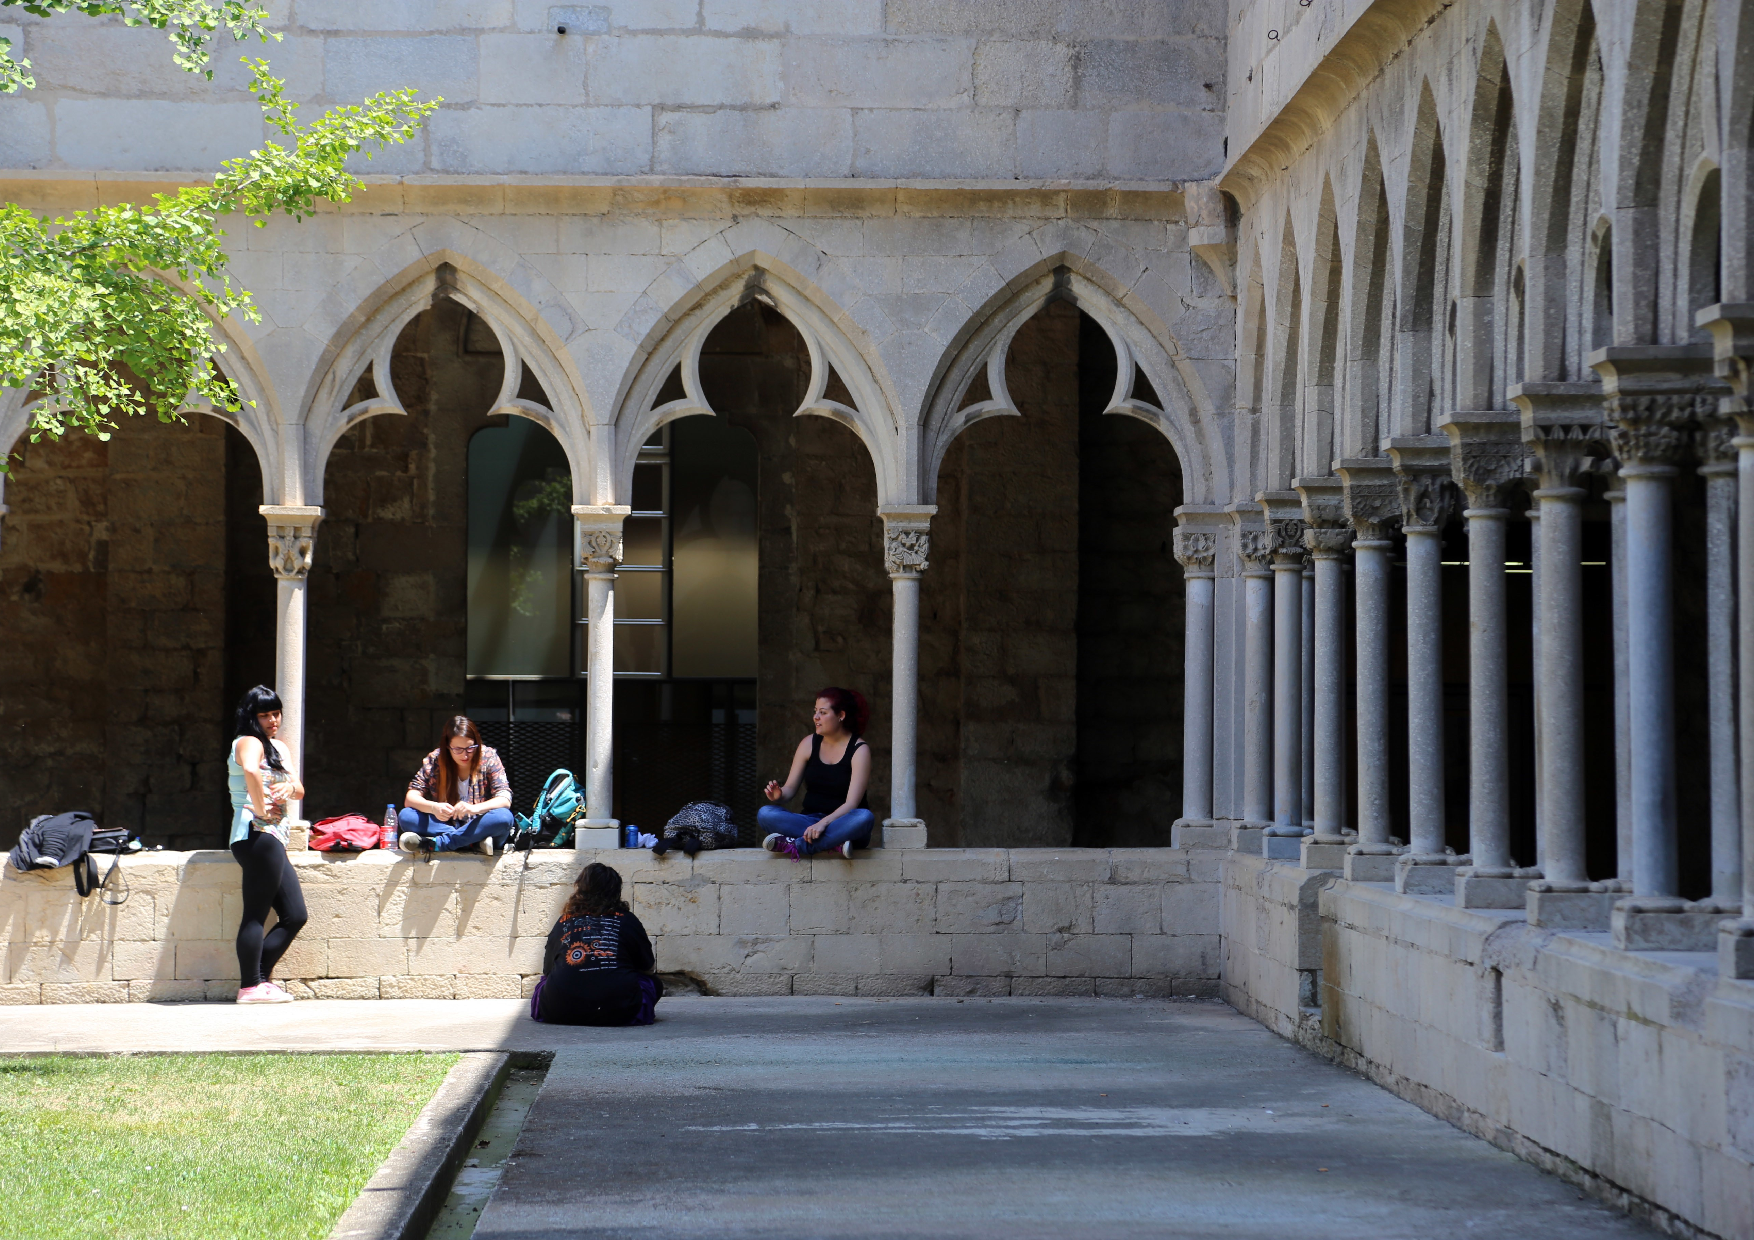
\includegraphics[width=0.55\linewidth]{Claustre.pdf}
\caption{The former cloister of the convent of St. Domènec, which is the venue of this conference.}
\label{fig:Claustre}
\end{figure}


Authors should upload the abstract via the website \texttt{composites2019.udg.edu} no later than \textbf{January 17, 2019}. 

\begin{thebibliography}{9}

% === Replace this by your references ===

\bibitem{Barbero} E.J. Barbero (2008) \textit{Finite Element Analysis of Composite Materials}. CRC Press, Boca Raton.
\bibitem{Pimenta} S. Pimenta and S.T. Pinho (2012) The effect of recycling on the mechanical response of carbon fibres and their composites. \textit{Composite Structures}, \textbf{94}, 3669-3684.

\end{thebibliography}
\end{document}
  
